\subsection{Statistical properties of syllable contact}

Above, we have seen that constraints on URs which are derive from phonological alternations restrict the contents of the lexicon. Applying these derived constraints to the lexicon increases saturation from 18.8\% to 28.8\% and incurs only a handful of exceptions. Yet, despite the fact that ``attestation'' is the minority pattern, attempts to identify static lexical constraints, whether by hand or computational model, lend little additional predictive power. There is no evidence that the English syllable contact inventory is subject to any static constraint at all. I am forced to conclude that most, if not all, of 71.2\% of possible clusters which are unattested are accidental gaps. Below, I show that this state of affairs follows directly from the sparse distribution of codas and onsets. 

\subsubsection{The $Z_r$ transform}

In a sparse distribution, many types occur at the same low frequencies. \citet{Good1953} notes that this produces a type of quantization, an artificially long and flat right tail in the frequency spectrum. \citet[][29]{Church1991} propose a method to eliminate this quantization, the $Z_r$ transform, defined as follows.
Let $r, n$ be defined such that $n_i$ is the number of types which occur at frequency $r_i$ (i.e., $n$ contains frequencies of type frequencies). Further, let $r$ be sorted in increasing order. $Z$ is simply each element of $n$ scaled by the nearest points to the left and right. 

\ex $\displaystyle Z_i = \frac{2 n_i}{r_{i + 1} - r_{i - 1}}$ \xe 

\noindent
\citeauthor{Church1991} do not define this transform for the lowest and highest points (i.e., when $i = 1$ or $i = N$), and so I extend the definition by scaling these points using only one inward-facing point.

\ex $\displaystyle Z_1 = \frac{n_1}{r_2 - r_1}$ \xe
\ex $\displaystyle Z_N = \frac{n_N}{r_N - r_{N - 1}}$ \xe

%\indent
%The effect of this transform can be seen in Figure \ref{zr}. 

%\begin{figure}
%\centering
%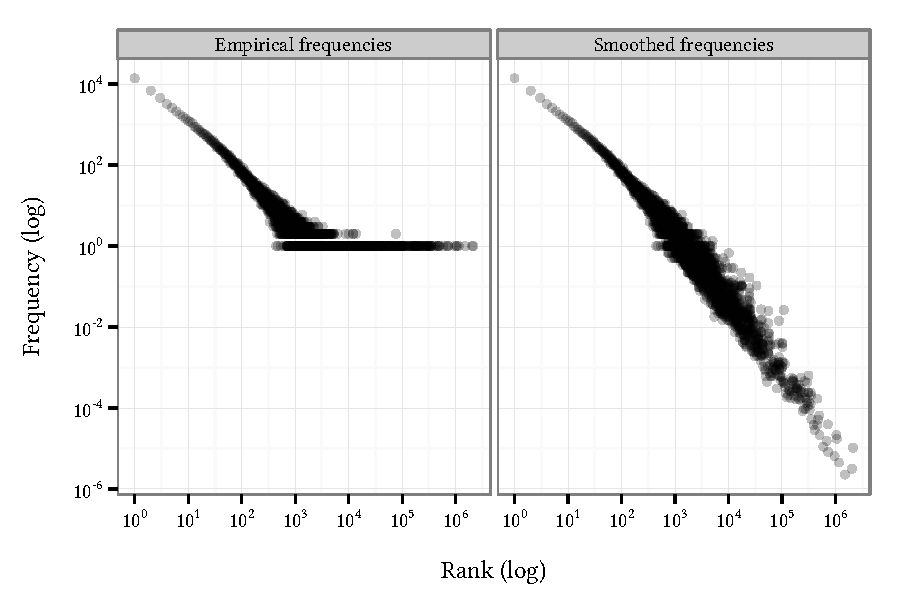
\includegraphics{zr.pdf}
%\caption{The SUBTLEX word frequency norms \citep{Brysbaert2009} show a long right tail in the log-frequency/log-rank space (left panel), and the $Z_r$ transform (right panel) smooths out this tail.}
%\label{zr}
%\end{figure}

\subsubsection{Coda, onset, and cluster sparsity}

A number of previous studies \citep[e.g.,][]{Sigurd1968,Good1969,Borodovsky1989,Witten1990,Martindale1996,Tambovtsev2007} have observed that phonemes and graphemes exhibit sparse type (i.e., lexical) and token frequency distributions. The lexical frequencies of the medial codas ond onsets which make up syllable contact clusters show a similar distribution. In Figure \ref{codaonset}, $Z_r$-transformed lexical frequencies of codas and onsets are plot against rank, in log-log spaces. The near-linear relationship that obtains indicates that the data can be modeled by a generalization of Zipf's law \citep{Zipf1949}.

\begin{figure}
\centering
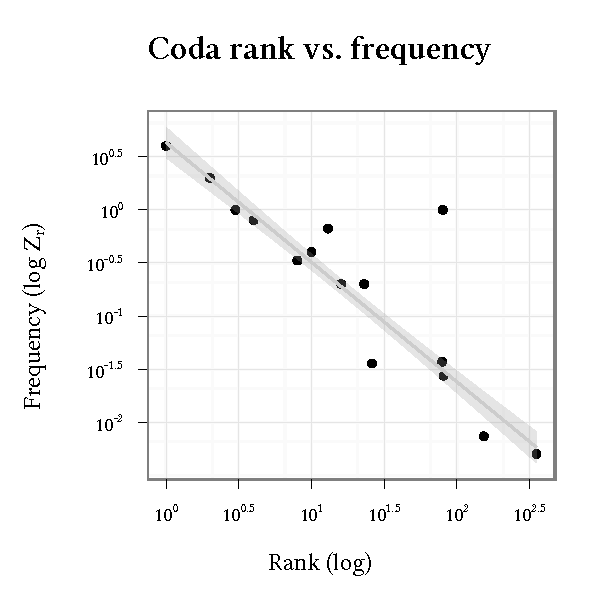
\includegraphics{coda.pdf} 
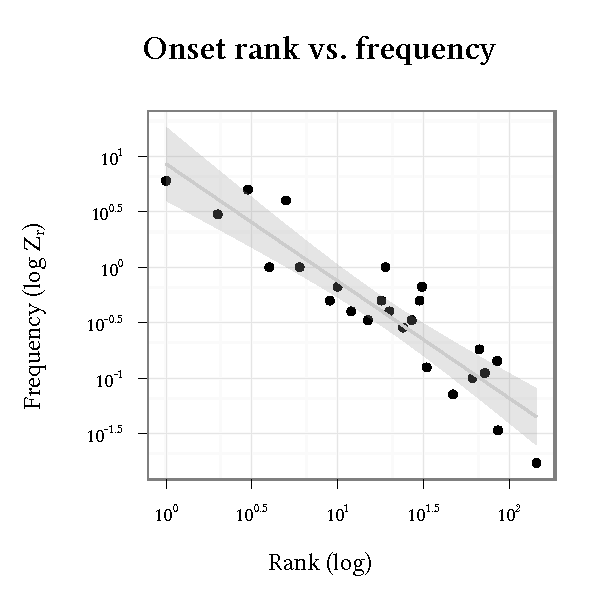
\includegraphics{onset.pdf}
\caption{Medial coda and medial onset lexical frequency exhibit the Zipfian log-log-linear relationship between rank and frequency.}
\label{codaonset}
\end{figure}

\ex $\displaystyle f(r; C, \alpha) = \frac{C}{r^\alpha}$ \xe

\noindent
The parameters $C$, a constant sensitive to sample size, and $\alpha$, the slope of the rank/frequency relationship in log-log space, are easily computed using the method of least squares in a linear regression, where $\epsilon$ represents the error term.

\ex $\displaystyle \textrm{log}~Z_r \sim C + \alpha~\textrm{log}~r + \epsilon$ \xe

\noindent
Codas ($\alpha = -0.720$, $R^2 = 0.749$) and onsets ($\alpha = -1.056$, $R^2 = 0.828$) are well-fit by this distribution, though there are some outliers. Similarly, clusters, shown in Figure \ref{clus}, are also a good fit to the generalized Zipf's law ($\alpha = -0.588$, $R^2 = 0.924$). 

\begin{figure}
\centering
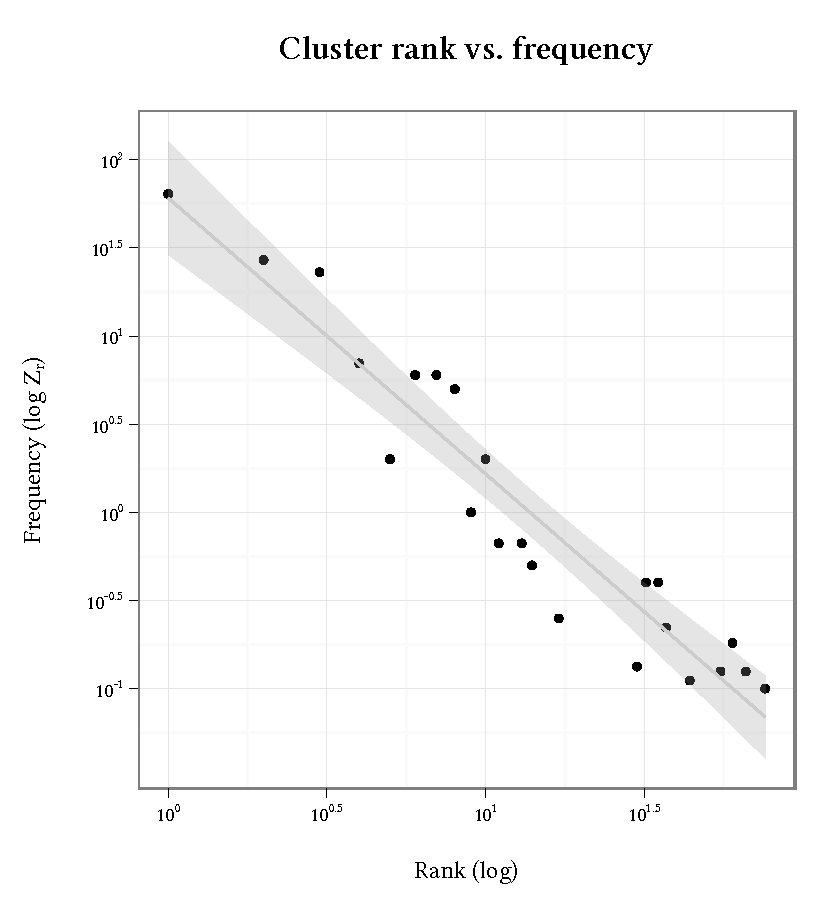
\includegraphics{cluster.pdf}
\caption{Syllable contact clusters, themselves composed of Zipfian medial codas and medial onsets, also exhibit a Zipfian distribution.}
\label{clus}
\end{figure}

That clusters (and the codas and onsets that make them up conforms to Zipf's law is not itself a deep observation. Zipfian distributions are characteristic of both syntactic rules \citep{Yang2009}, but also word \citep{Baroni2009} and phoneme \citep{Daland2011a} n-grams, and tokens in non-linguistic symbol systems \citep{Chomsky1958,Sproat2010} or randomly-generated texts \citep{Miller1957,Li1992}. The import of this statistical property for the study of cluster phonotactics is that it makes it difficult, on statistical grounds alone, to determine which unobserved events are excluded, and which are accidentally missing. 

\citet{Good1953} puts forth a simple theory of just how frequent unobserved events might be. He proposes to estimate $\hat{p}_0$, the probability of all unseen events, as the ratio of events which occur just once $n_1$, to the number of observations, $\sum N$. This quantity is known as the Good-Turing estimate, since it was originally developed by Alan Turing for codebreaking during the second World War.

\ex $\displaystyle \hat{p}_0 = \frac{n_1}{\sum N}$ \xe

\noindent
In the CELEX data, $65$ clusters occur only once, and there are 873 clusters in all, so $\hat{p}_0 = 0.074$. One way to interpret this quantity is with respect to a ``replication''. If it were possible to generate a new corpus of syllable contact clusters, approximately 7\% of cluster tokens will be ones that were not attested in the previous sample, i.e., they accidentally failed to be sampled. This is a not-inconsiderable quantity. 

Unfortunately, the Good-Turing estimate does not provide a way to determine which unattested clusters might be found in a replication. But I have already proposed that the null hypothesis of generative phonology, combined with the principle of Stampean occultation, provides a way out of this conundrum. Unattested clusters like *[m.kl] are structurally excluded (since such a cluster is occulted by \textsc{Coda Nasal Place Assimilation}), whereas *[s.l] is probably an accidental gap.

\subsubsection{Sampling simulation}

As a final investigation into this data, I consider the statistical properties of a randomly generated novel ``lexicon''. The simulated lexicon is generated by  generating a distribution of clusters, by repeatedly applying the following procedure.

\ex {Simulation procedure}: \\
    \begin{tabular}{l l}
    a. & Sample a medial coda according to the observed probabilities  \\
    b. & Sample a medial onset according to the observed probabilities \\
    c. & Apply the SPE rules to the resulting cluster                  \\
    \end{tabular}
\xe

\noindent
This is a simulation version of the model proposed by \citet{Pierrehumbert1994} and \citet{Coleman1997}, but also takes occulting phonology into account. 

While this procedure can be repeated indefinitely (using the CELEX data, listed in Appendix \ref{A}), consideration of a single characteristic run of the simulation should suffice. The saturation rate of the simulated sample (18.2\%) is very close to the real sample (18.8\%). The slope of the log-rank/log-frequency relationship for the simulated data ($\alpha = -0.557$) is also very close to the observed slope for the CELEX data ($\alpha = -0.588$). And, as shown in Figure \ref{sim}, the two distributions are nearly indistinguishable. 

\begin{figure}
\centering
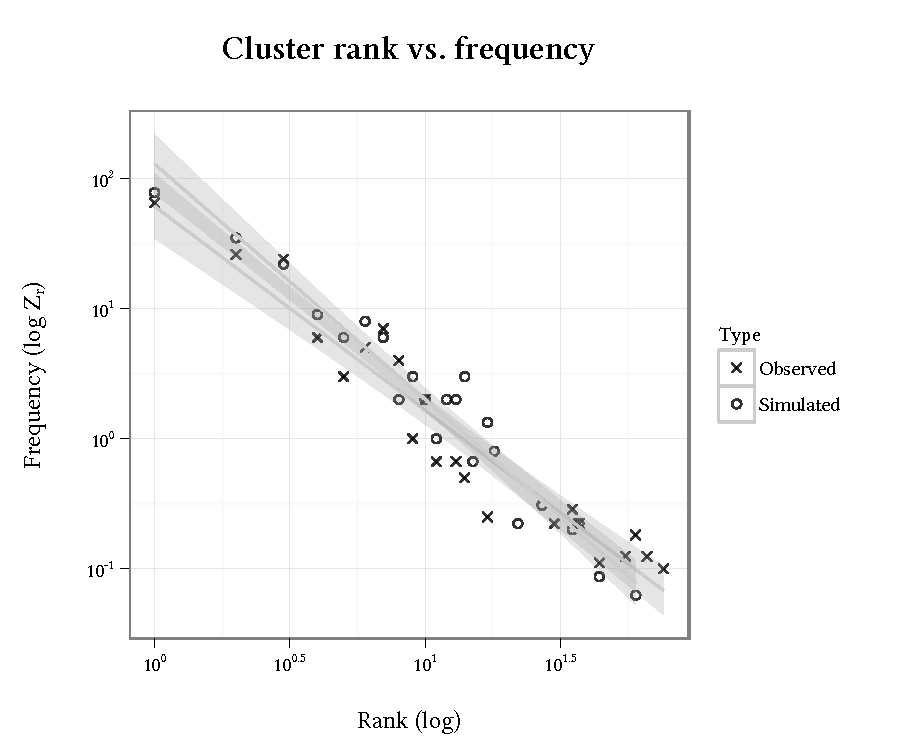
\includegraphics{sim.pdf}
\caption{A comparison of the observed lexical frequencies of English syllable contact clusters to an ``English lexicon'' simulated by combining.}
\label{sim}
\end{figure}

It is important to note that the results of this simulation should not be construed as an endorsement of a revised version of the \citet{Pierrehumbert1994} and \citet{Coleman1997} model which also incorporates occultation. In fact, as was shown above, the independent frequencies of coda and onset are very poor predictors of what clusters will be attested even when occultation is taken into account, and the set of attested clusters only partially overlaps those produced by the simulation. I propose that this is because the lexicon is not only finite, but far smaller than the combinatoric possibilities provided by phoneme sequences, making accidental gaps unavoidable. That these gaps will be arbitary from the perspective of phonology is nothing more than a corrolary of the principle of \emph{l'arbitraire du signe}. 

It is quite possible that phonology (and, perhaps, static phonotactics) acts as a filter on what URs are learned, but a cluster might be overrepresented or underrepresented for reasons that are quite external to phonology, e.g., language contact or historical change. Similarly, the factors that cause a /n/ to be a common word-medial coda in English may be independent of the propensity of that coda to combine with medial onset, assuming the resulting cluster is phonologically licit. The import of this simulation is somewhat more subtle; it simply shows free combination of codas and onsets according to their independent probabilities, constrained only by occultation, would produce the same sparse distribution of clusters that was used to argue for static phonotactics.

%\citet{Evert2004}
%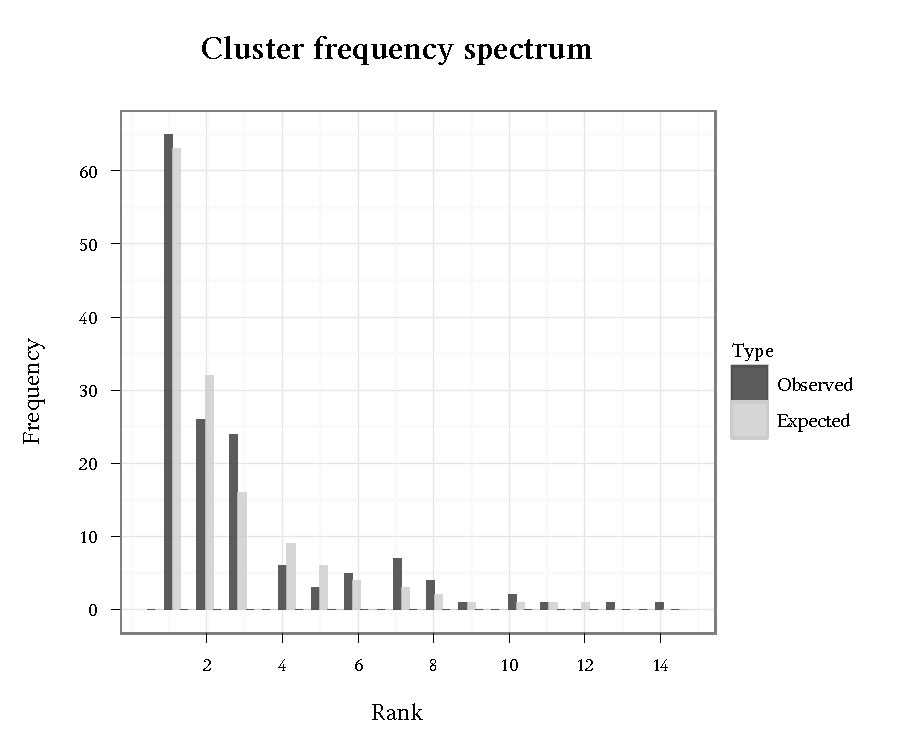
\includegraphics{zipf.pdf}
